\section{Krylow-Verfahren für LGS}
\subsection{Grundlagen, Arnoldi}

\begin{karte}{Krylow-Raum}
    Zu \( A\in \C^{n,n} \) und \(b\in \C^n, b\neq 0 \), 
    heißt 
    \[ \Kcal_m(A,b) = \spann\set{b, Ab, \ldots, A^{m-1}b} \]
    der \(m\)-te \textit{Krylow-Raum} bezüglich \(A\) und \(b\).
\end{karte}

\begin{karte}{Konstruktion Krylow-Raum}
    Ist \(V_j \in \C^{n,j}\) eine Basis für \( \Kcal_j \) für \(j = 1,\ldots, m+1\), 
    wobei \( V_j = [V_{j-1} v_j] \), dann gibt es eine eindeutig bestimmte 
    nicht reduzierte obere Hessenbergmatrix \( \tilde{H}_m = (h_{ij}) \in \C^{m+1,m} \), 
    sodass 
    \[ A V_m = V_{m+1} \tilde{H}_m. \]
\end{karte}

\begin{karte}{Arnoldi-Algorithmus}
    \begin{tabbing}
        Zu gegebenem \(A\in \C^{n,n}, b\in \C^n\), berechne \( \beta = ||b||>0 \) \\
        \(v_1 = b/\beta\) \\
        for \= \( m = 1,2,\ldots \) do \\
        \> for \= \(j = 1,\ldots, m \) do \\
        \> \> \( h_{j,m} = v_j^H A v_m \) \\
        \> end for \\
        \> \( \tilde{v}_{m+1} = A v_m - \sum_{j=1}^m h_{j,m} v_j \) \\
        \> \( h_{m+1,m} = ||\tilde{v}_{m+1}|| \) \\
        \> \( v_{m+1} = \tilde{v}_{m+1}/h_{m+1,m} \) \\
        end for
    \end{tabbing}
    Unterschied zwischen Arnoldi und Gram-Schmidt: im \(m\)-ten Schritt wird
    nicht \( A^m b\) sondern \(A v_m\) verwendet. Dies ist mathematisch äquivalent, 
    allerdings aus Stabilitätsgründen zu bevorzugen.
\end{karte}

\begin{karte}{Eigenschaften Arnoldi-Verfahren}
    Seien \(V_m\) und \( \tilde{H}_m \) die Matrizen aus dem Arnoldi-Verfahren. 
    Dann gilt 
    \begin{enumerate}
        \item \( V_m^H V_m = I_m \),
        \item \( A V_m = V_{m+1} \tilde{H}_m = V_m H_m + h_{m+1,m} v_{m+1} e_m^T \),
        \item \( V_m^H A V_m = H_m \),
        \item \( V_{m+1}^H A V_m = \tilde{H}_m \),
        \item Für \( A = A^H \) ist \( H_m = H_m^H \) tridiagonal.
    \end{enumerate}
    \begin{tabular}{|c|c|c|}
        \hline
        Berechnung von & \(A\) beliebig & \(A\) hermitesch \\
        \hline
        \(A v_m\) & \(1\) Matrix-Vektormult. & \(1\) Matrix-Vektormult. \\
        \( h_{j,m} \) & \(m\) Skalarprodukte & \(1\) Skalarprodukt (\(h_{m-1,m} = \overline{h_{m,m-1}}\)) \\
        \( \tilde{v}_{m+1} \) & \(m\) \textsc{SAXPYs} & \(2\) \textsc{SAXPYs} \\
        \( h_{m+1,m} \) & \(1\) Skalarprodukt & \(1\) Skalarprodukt \\
        \( v_{m+1} \) & \(n\) Divisionen & \(n\) Divisionen \\\hline
        Speicher & \(m+1\) Vektoren & \(3\) Vektoren\\
        \hline
    \end{tabular}
\end{karte}

\begin{karte}{Abbruch Arnoldi-Prozess}
    Der Arnoldi-Algorithmus bricht ab, wenn \( h_{m+1,m} = 0 \) 
    bzw. \( A V_m = V_m H_m \) ist. Dann enthält der bisher konstruierte 
    Krylow-Raum bereits die exakte Lösung \( \widehat{x} = A^{-1}b \), d. h. 
    es existiert ein \( y_m \in \C^m \), sodass \( \widehat{x} = A^{-1}b = V_m y_m \).

    Beste Approximation: \(y_m\) soll Fehler \( f_m = \widehat{x} - x_m \)
    in einer gegebenen Norm \(||\cdot||\) minimieren: 
    \[ ||f_m|| = \min_{x\in \Kcal_m} ||\widehat{x} - x||. \]
\end{karte}

\begin{karte}{Residuenvektor}
    Sei \( r_m = A(\widehat{x} - x_m) \). 

    Es gilt \begin{align*}
        r_m &= b - A V_m y_m \\ 
        &= \beta v_1 - V_{m+1} \tilde{H}_m y_m \\
        &= V_{m+1} (\beta e_1 - \tilde{H}_m y_m).
    \end{align*}

    Also folgt 
    \[ ||r_m|| = ||V_{m+1}(\beta e_1 - \tilde{H}_m y_m)|| \leq ||V_{m+1}|| \;||\beta e_1 - \tilde{H}_m y_m||. \]

    \gqq{\(=\)}, wenn \(V_{m+1}\) unitär.
\end{karte}

\begin{karte}{Charakterisierung von \(y_m\)}
    (M): Minimiere \( ||\beta e_1 - \tilde{H}_m y|| \) über alle \(y \in \C^m\). 
    Dies führt auf ein lineares Ausgleichsproblem der Dimension \((m+1)\times m\). 
    \[ y_m = \beta (\tilde{H}_m^H \tilde{H}_m)^{-1} \tilde{H}_m^H e_1 = \beta \tilde{H}_m^+ e_1, \]
    wobei \( \tilde{H}_m^+ \) die Pseudoinverse von \( \tilde{H}_m \) bezeichnet.

    (G): Wähle \(y_m\) so, dass \(r_m\) orthogonal zu einem geeigneten Unterraum 
    \( \mathcal{W}_m \) der Dimension \(m\) ist. Für \( \mathcal{W}_m = \Kcal_m \)
    heißt die Bedingung \textit{Galerkin-Bedingung}, ansonsten \textit{Petrov-Galerkin-Bedingung}.
\end{karte}

\begin{karte}{(M) und (G) liefern eine Lösung}
    Ist \(A V_m = V_m H_m\) und ist \(W_m\) eine Basis von 
    \( \mathcal{W}_m \) mit \(W_m^H V_m\) nicht singulär, dann 
    ist \( x_m = V_m y_m \), wobei \(y_m\) durch (M) oder (G) charakterisiert ist, 
    die exakte Lösung, d. h. \( x_m = \widehat{x} = A^{-1}b \).

    Alle Krylov-Verfahren, deren Iterierte durch (M) oder (G) 
    bestimmt sind, liefern nach höchstens \(n\) Schritten die exakte Lösung.
\end{karte}

\subsection{Verfahren mit Arnoldi}

\begin{karte}{Residuenvektor Abschätzung}
    Ist \( V_{m+1} \) unitär und \(y_m = \beta \tilde{H}_m^+ e_1\) die Lösung 
    von (M), dann erfüllt \( x_m = V_m y_m \)
    \[ ||r_m|| = ||b - A x_m|| \leq ||b - Ax|| \quad \forall x\in \Kcal_m. \]
\end{karte}

\begin{karte}{GMRES}
    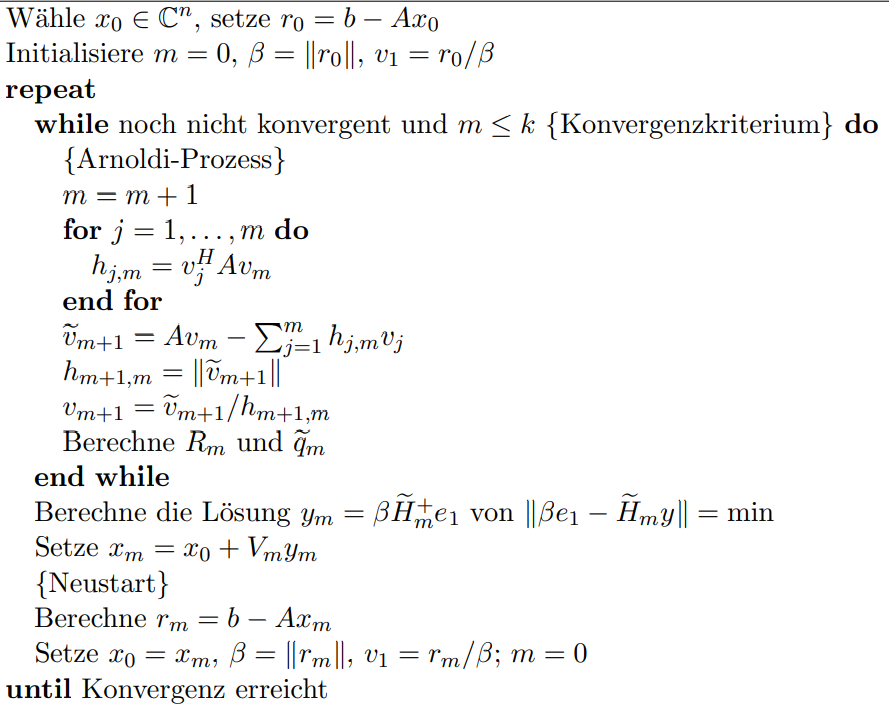
\includegraphics[width=0.8\textwidth]{GMRES.png}
\end{karte}

\begin{karte}{GMRES, FOM Eigenschaften}
    GMRES(\(k\)) wird nach \(k\) Iterationen neugestartet, falls der Speicherverbrauch 
    zu groß wird.
    Hierbei geht die Minimierungseigenschaft verloren und somit verlangsamt sich die Konvergenz.

    FOM ist die Galerkin-Bedingung kombiniert mit dem Arnoldi-Algorithmus. 
    Auch diese Variante kann neu gestartet werden.

    Sei \( V_{m+1} \) unitär und \( \mathcal{W}_m = \Kcal_m \). Dann 
    existiert eine Lösung von (G) genau dann, wenn \(H_m\) nicht singulär ist. 
    In diesem Fall ist \(x_m = V_m y_m\), wobei \(H_m y_m = \beta e_1\).
\end{karte}

\begin{karte}{Wertebereich \( H_m \)}
    Ist \(V_m\) unitär, dann gilt 
    \( \mathcal{F}(H_m) \subseteq \mathcal{F}(A) \). Insbesondere folgt aus
    \( 0 \notin \mathcal{F}(A) \), dass \( H_m \) für alle \(m\) nicht singulär ist.
\end{karte}

\begin{karte}{Wünschenswerte Eigenschaften eines Krylowverfahrens}
    Wünschenswert sind
    \begin{enumerate}
        \item Minimierung des Fehlers (oder Residuums) in einer festen Norm unabhängig vom Startwert
        \item kurze Rekursionen (gleicher Aufwand in jedem Schritt)
    \end{enumerate}

    Es ist i. A. nicht möglich, beides gleichzeitig zu erfüllen. 
    GMRES erfüllt 1., jedoch nicht 2., FOM erfüllt weder 1. noch 2..
    Das nichtsymmetrische Lanczos-Verfahren erfüllt 2. und 1. in einer abgeschwächten Form.
\end{karte}

\subsection{Nichtsymm. Lanczos-Verfahren}

\begin{karte}{Nichtsymmetrisches Lanczos-Verfahren Grundprinzip}
    Man berechnet eine Basis \( (v_j)_j \) von \( \Kcal_m(A,b) \)
    und eine Basis \( (w_j)_j \) von \( \Kcal_m(A^H, c) \) für einen geeigneten 
    Vektor \(c\in \C^n\). 

    Wir verlangen außerdem Biorthogonalität der beiden Basen:
    \[ w_j^H v_k = \begin{cases}
        0, & j\neq k, \\ \delta_k \neq 0, & j = k,
    \end{cases} \]
    oder 
    \[ v_m \bot \Kcal_{m-1}(A^H, c), \quad w_m \bot \Kcal_{m-1}(A, b). \]
\end{karte}

\begin{karte}{Nichtsymmetrisches Lanczos-Verfahren}
    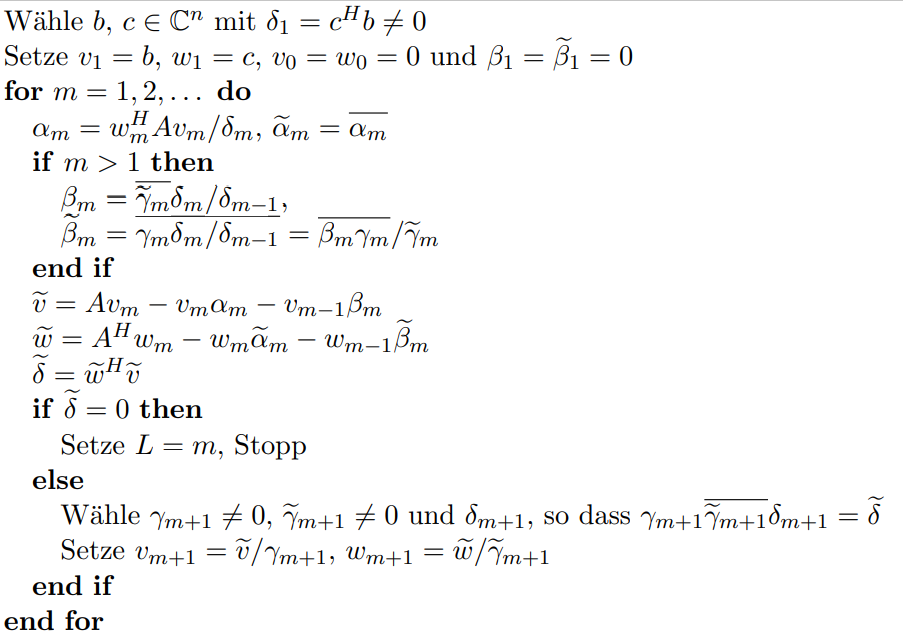
\includegraphics[width=0.8\textwidth]{Nichtsymmetrisches-Lanczos-Verfahren.png}
\end{karte}

\begin{karte}{Nichtsymmetrisches Lanczos-Verfahren Eigenschaften}
    Für das nichtsymmetrische Lanczos-Verfahren gilt 
    \begin{enumerate}
        \item \( W_m^H V_m = D_m = \diag(\delta_1, \ldots, \delta_m), m = 1,\ldots, L \),
        \item \( A V_m = V_{m+1} \tilde{T}_m = V_m T_m + \gamma_{m+1} v_{m+1} e_m^T \),
        \item \( A^H W_m = W_{m+1} \tilde{S}_m = W_m S_m + \tilde{\gamma}_{m+1} w_{m+1} e_m^T \), 
        wobei \(\tilde{S}_m\) analog zu \(\tilde{T}_m\) definiert ist, jedoch mit Koeffizienten 
        \( \tilde{\alpha}_j, \tilde{\beta}_j, \tilde{\gamma}_j \), 
        \item \( W_m^H A V_m = D_m T_m = S_m^H D_m \),
        \item in exakter Arithmetik bricht der Lanczos-Prozess nach \(m= L-1\) 
        Schritten ab, wobei 
        \[ 1 \leq L \leq \min\set{ \dim \Kcal_n(A,b), \dim \Kcal_n(A^H, c) }. \]
    \end{enumerate}
\end{karte}

\begin{karte}{Zusammenbruch}
    Der Lanczos-Algorithmus bricht ab, wenn 
    \( \tilde{\delta} = \tilde{w}_L^H \tilde{v}_L = 0 \). 
    Hierfür gibt es zwei verschiedene Ursachen:
    \begin{description}
        \item[Regulärer Zusammenbruch] \( \tilde{w}_L = 0 \) 
        oder \( \tilde{v}_L = 0\). Ist \( \tilde{w}_l = 0 \), 
        dann spannen die linken Lanczos-Vektoren einen \(A^H\)-invarianten 
        Unterraum auf, sonst spannen die rechten Lanczos-Vektoren einen 
        \(A\)-invarianten Unterraum auf.
        \item[Ernsthafter Zusammenbruch] \( \tilde{w}_l \neq 0 \neq \tilde{v}_L \). 
        Die Lanczos-Vektoren spannen weder einen \(A\)- noch einen \(A^H\)-invarianten 
        Unterraum auf.
    \end{description}
\end{karte}

\subsection{Konjugierte Gradienten}

\begin{karte}{Allgemeines zum Galerkin-Verfahren}
    Wenn die Koeffizientenmatrix hermitesch und 
    positiv definit ist, dann können wir beim Lanczos-Verfahren 
    einfach zwei Basen für \( \Kcal_m(A, b) \) 
    und \( \Kcal(A, r_0) \) berechnen. 

    Das so definierte Galerkin-Verfahren ist für \( A = A^H \)
    positiv definit und ein Minimierungsverfahren in 
    der Energienorm \(||x||_A = \sqrt{x^H Ax}\).
\end{karte}

\begin{karte}{Fehlerabschätzung cg-Verfahren 1}
    Ist \( \widehat{x} = A^{-1}b \) die Lösung 
    des LGS \(Ax=b\), \(A = A^H\) positiv definit, 
    \(x_m \in x_0 + \Kcal_m(A,r_0)\) 
    die Galerkin-Iterierte (\(r_m \bot \Kcal_m(A, r_0)\)),
    dann gilt für die Iterierten \(x_m\) des cg-Verfahrens 
    \[ ||\widehat{x} - x_m||_A \leq ||\widehat{x} - x||_A \]
    und 
    \[ ||b - A x_m||_{A^{-1}} \leq ||b-Ax||_{A^{-1}} \]
    für alle \(x \in x_0 + \Kcal_m(A, r_0)\).
\end{karte}

\begin{karte}{Fehlerabschätzung cg-Verfahren 2}
    Ist \(A = A^H\) positiv definit, so gilt für den Fehler 
    der \(m\)-ten Iterierten des cg-Verfahrens 
    \[ ||x_m - \widehat{x}||_A \leq \min_{\substack{p_m \in \mathcal{P}_m \\ p_m(0) = 1}} 
    ||p_m(A)|| \; ||x_0 - \widehat{x}||_A. \]

    Außerdem gilt 
    \[ \min_{\substack{p_m \in \mathcal{P}_m \\ p_m(0) = 1}} 
    ||p_m(A)|| \leq 2 \left( \frac{\sqrt{\kappa} - 1}{\sqrt{\kappa} + 1} \right)^m, \]
    wobei \(\kappa = \kappa(A) = ||A|| \cdot ||A^+||\) die Konditionszahl von \(A\) bezeichnet.
\end{karte}

\begin{karte}{cg-Verfahren aus Lanczos-Verfahren}
    Man kann das cg-Verfahren direkt über das Lanczos-Verfahren herleiten: 
    Für gegebenes \(x_0\) und \(r_0 = p_1 = b - Ax_0\) 
    verwendetn wir für \( m=1,2,\ldots \) den Ansatz 
    \begin{align*}
        x_m &= x_{m-1} + \tau_m p_m, \\
        r_m &= r_{m-1} - \tau_m A p_m, \\
        p_{m+1} &= r_m - \mu_{m+1} p_m.
    \end{align*}
\end{karte}

\begin{karte}{cg-Verfahren Eigenschaften}
    Für die Vektoren aus dem cg-Verfahren gilt: 
    \begin{enumerate}
        \item \(r_m\) ist Residuenvektor zu \(x_m\), \(r_m = b - A x_m\).
        \item Die Residuenvektoren \( r_0, \ldots, r_m \) und die Suchrichtungen 
        \(p_1, \ldots, p_m\) des cg-Verfahrens erfüllen 
        für \( m \leq \dim \Kcal_n(A, r_0) \), falls \(\tau_j \neq 0, j=1,\ldots, m\), 
        \[ \spann\set{ r_0,\ldots, r_{m-1} } = 
        \spann\set{p_1, \ldots, p_m} = \Kcal_m(A, r_0). \]
        \item Wählt man 
        \[ \tau_m = \frac{r_{m-1}^H r_{m-1}}{ p_m^H A p_m} = \frac{\delta_m}{\delta_m'} \]
        und 
        \[ \mu_{m+1} = \frac{p_m^H A r_m}{p_m^H A p_m} = - \frac{r_m^H r_m}{r_{m-1}^H r_{m-1}} = - \frac{\delta_{m+1}}{\delta_m}, \]
        so sind Residuenvektoren orthogonal, \( r_k^H r_j = 0 \) 
        für \(j\neq k\) und die Suchrichtungen \(A\)-konjugiert, 
        \(p_k^H A p_j = 0, j \neq k\). Insbesondere ist \(x_m\) die
        cg-Iterierte.
    \end{enumerate}
\end{karte}

\begin{karte}{cg-Verfahren}
    \begin{tabbing}
        Wähle \( x_0 \in \C^n \), setze \(r_0 = b - A x_0\) und wähle Toleranz \(\texttt{tol} > 0\) \\
        Initialisiere \(m = 1, p_1 = r_0, \delta_1 = r_0^H r_0\) \\
        while \= \(\delta_m \geq \texttt{tol}^2 \) do \\
        \> Berechne \(\delta_m' = p_m^H A p_m\) \\
        \> Berechne \(\tau_m = \delta_m / \delta_m'\) \\
        \> Setze \(x_m = x_{m-1} + \tau_m p_m\) \\
        \> Berechne \(r_m = r_{m-1} - \tau_m A p_m\) \\
        \> Berechne \( \delta_{m+1} = r_m^H r_m, \mu_{m+1} = -\delta_{m+1}/\delta_m \) \\
        \> Setze \( p_{m+1} = r_m - \mu_{m+1} p_m \) \\
        \> Ersetze \(m\) durch \(m+1\) 
        end while
    \end{tabbing}
    Das cg-Verfahren bewirkt eine schnelle Fehlerreduktion, 
    wenn die Kondition von \(A\) klein ist oder die Eigenwerte 
    von \(A\) in eineigen wenigen Clustern liegen.

    Falls die Eigenschaften diese Eigenschaften nicht haben, 
    kann man mit einem äquivalenten LGS mit besseren Eigenschaften 
    arbeiten (Vorkonditionierung).
\end{karte}

\subsection{Basierend auf Lanczos}

\begin{karte}{QMR-Verfahren (quasi minimal residual method)}
    Lanczos-Verfahren mit (M)-Bedingung
    \begin{tabbing}
        Wähle \( x_0 \in \C^n \), setze \(r_0 = b - A x_0, \beta = \rho_0 = ||r_0||\) \\
        Setze \( p_0 = p_{-1} = 0 \)  \\
        Starte den nichtsymmetrischen Lanczos-Prozess mit geeignetem \\
        linken Startvektor \(c\) und \(v_1 = r_0/\beta\) \\
        Am Ende \= des \(m\)-ten Schritts ergänze folgende Zeilen:\\
        \> Berechne \( \theta_m, \eta_m, \zeta_m, \rho_m, \tau_m \) \\
        \> Setze \( p_m = (v_m - \eta_m p_{m-1} - \theta_m p_{m-2})/\zeta_m \) \\
        \> Berechne \( x_m = x_{m-1} + \tau_m p_m \)
    \end{tabbing}
    Kosten sind sieben \textsc{SAXPYs}, zwei Skalarprodukte \\
    und zwei Matrix-Vektormultiplikationen pro Schritt.
\end{karte}

\begin{karte}{Lösung für Koeffizienten des BiCG-Verfahrens}
    Seien \(V_m, W_m\) die Matrizen aus dem Lanczos-Prozess 
    und \(x_m = V_m y_m\). Dann existiert eine Lösung von (G) 
    genau dann, wenn \(T_m\) nicht singulär ist. In diesem Fall ist 
    \(T_m y_m = \beta e_1\).
\end{karte}

\begin{karte}{BiCG-Verfahren Vektoren}
    Führen wir wie bei QMR Suchrichtungen ein, so erreichen wir die 
    kurze Rekursion für \(x_m\): Wegen \( T_m^{-1} = U_m^{-1} E_m^{1} L_m^{-1} \) gilt 
    \[ x_m = P_m z_m, \quad P_m = V_m U_m^{-1}, \quad z_m = \beta E_m^{-1} L_m^{-1} e_1. \]
    Wir können \(p_m\) mit einer Rekursionsformel berechnen: 
    \[ p_1 = v_1, \quad p_m = v_m - \mu_m p_{m-1}.\]

    Zu gewissen Indizes können evtl. keine Iterierten existieren, die (G) 
    erfüllen. Man kann um schlechte/instabile Iterierte vermeiden, 
    indem man die BiCG-Iterierten aus QMR-Iterierten berechnet. 
\end{karte}

\begin{karte}{BiCG-Verfahren (biconjugate gradient method)}
    \begin{tabbing}
        Wähle \( x_0 \in \C^n \), setze \(r_0 = b - A x_0, \beta = \rho_0 = ||r_0||\) \\
        Setze \( p_0 = p_{-1} = 0 \)  \\
        Starte den nichtsymmetrischen Lanczos-Prozess mit geeignetem \\ 
        linken Startvektor \(c\) und \(v_1 = r_0/\beta\) \\
        Am Ende des \(m\)-ten Schritts ergänze folgende Zeilen:\\
        if \= \(m=1\) then \\
        \> \(\varepsilon_1 = \alpha_1, \tau_1 = \beta/\varepsilon_1\) \\
        else \\
        \> {Berechne den Update der LDU-Zerlegung von \(T_m\)} \\
        \> \( \nu_m = \gamma_m/\varepsilon_{m-1}, \mu_m = \beta_m / \varepsilon_{m-1}, \varepsilon_m = \alpha_m - \nu_m \beta_m \) \\
        \> Setze \( \tau_m = -\varepsilon_{m-1} \tau_{m-1} \nu_m / \varepsilon_m \) \\
        \> Berechne \( p_m = v_m - \mu_m p_{m-1} \) \\
        end if \\
        Berechne \(x_m = x_{m-1} + \tau_m p_m\)
    \end{tabbing}

    Aufwand: pro Schritt sechs \textsc{SAXPYs}, zwei Skalarprodukte und 
    zwei Matrix-Vektormultiplikationen.
\end{karte}

\subsection{Vorkonditionierung}

\begin{karte}{Idee Vorkonditionierung}
    LGS kann näherungsweise gelöst werden. 
    Konvergenz hängt wesentlich von der Lage 
    der Eigenwerte oder des Wertebereichs ab. 

    \[ A x = b \Leftrightarrow BAx = Bb. \]
    \(B = A^{-1}\) wäre die optimale Wahl (Konvergenz in einem Schritt).

    Wir verlangen für den Vorkonditionierer
    \begin{enumerate}
        \item \(B \approx A^{-1}\),
        \item \( B \in \R^{n,n} \) symmetrisch und positiv,
        \item \(x \mapsto Bx\) leicht zu berechnen.
    \end{enumerate}   
\end{karte}

\begin{karte}{Unvollständige Cholesky-Zerlegung}
    Wählen die Faktorisierung \( A = \tilde{L} \tilde{L}^T + R \), 
    wobei \(\tilde{L}\) eine untere Dreiecksmatrix mit derselben Besetzungsstruktur 
    wie \(A\) und \(R\) eine Restmatrix.

    Häufig bewirkt \( B = (\tilde{L} \tilde{L}^T)^{-1} \) eine Clusterung 
    der Eigenwerte von \(BA\).

    Wenn eine Faktorisierung von \(B = C C^T\) von \(B\) bekannt ist, 
    (z. B. \(C = \tilde{L}^{-T}\)), ist unser neues LGS auch positiv definit: 
    \[ B Ax = Bb \Leftrightarrow C C^T A x = C C^T b \Leftrightarrow \tilde{A} \tilde{x} = \tilde{b} \]
    mit \( \tilde{A} = C^T A C, \tilde{x} = C^{-1} x, \tilde{b} = C^T b \).
\end{karte}

\begin{karte}{Fehlerabschätzung Vorkonditionierung}
    Angenommen, es existieren \( 0 < \gamma \leq \Gamma \) mit 
    \[ \gamma v^T B^{-1} v \leq v^T A v \leq \Gamma v^T B^{-1} v \quad \forall v\in\R^n. \]
    Ist \( \widehat{x} = x^* = A^{-1}b \), dann gilt die Fehlerabschätzung 
    \[ ||x_m - x^*||_A \leq 2 \left( \frac{\sqrt{\tilde{\kappa}} - 1}{\sqrt{\tilde{\kappa}} + 1} \right)^m 
    ||x_0 - x^*||_A \quad, \tilde{\kappa} = \frac{\Gamma}{\gamma}. \]
\end{karte}